% !TEX root = ../paper.tex
\section{Discussion}
Our results have shown that our semantic similarity is practical to assist in reducing effort and error proneness of manual assessment of comment usefulness.  
Besides this result, we also found some noteworthy findings in our case study:

% tuning the F score for precision and recall
%Depending on the use case, we can fine-tune the F-score to give more weight to recall or precision.
%For instance, if we wanted to measure the amount of useful comments within a large dataset, more weight can be given to precision, sacrificing some useful comments.
%If we wanted to modify a code review software such that it displays useful comments more prominently, more weight can be given to recall.

% examples.
\subsection{What kind of comments cannot be classified using semantic similarity?}

From the results of RQ1, we found that some comments were not determined by our model.
Specifically, we were interested in why some manually assessed useful comments (\texttt{YES} = 3) and useless comments (\texttt{YES} = 0) were undetermined.
To investigate the reason behind this, we reviewed these comments and the corresponding commit messages.
We found that there were few common keywords between the comments and commit messages and their lengths are relatively unequal.
This makes for low similarity values and low dissimilarity values as shown in bottom left white area in Fig. \ref{fig:scatter}. There simply isn't enough semantic information to determine anything.


%In some cases, similarity and dissimilarity failed to measure the usefulness of the comment,
%due to the same word being used in a different context.
%For example, consider this excerpt from the commit message: \emph{``In the no-assert case, make Q\_ASSERT decay to Q\_ASSUME. I can confirm
%better code generation with GCC at least.''}
%This comment, \emph{``I'll study the generated code a bit more,''} is just an author's response, and thus is not technically contributing. However, it is classified as a useful comment. This may be caused by the word \emph{generate} which appears in both documents.


%\subsection{Binary Classification}
%\subsection{How much impact of unclear class on model construction?}
%\pick{This topic of discuss should be changed....}
% % noisy data, and binary classification
%
% 
% 
%Our training data contains much variability because there are disagreements between our judgment of ``usefulness,'' rendering our results unclear; they cannot be classified as either useful or not useful.
%This impacts the trade-off between the precision and recall for our model, and consequently, the F$_1$ score.
%
%Another approach we tried is to perform a \emph{binary classification}.
%This means we assume that there are no unclear or undetermined comments; only useful and useless.
%For this, we removed the samples with 1 and 2 \texttt{YES} votes from our training set.
%This leaves us with 209 remaining samples, all without a disagreement.
%By performing cross-validation using these samples, we obtained a much better F$_1$ score of 0.896.
%
%However, we could not objectively measure the F$_1$ score for all samples, because giving positive or negative classification to 1 and 2-scored samples introduces a bias.
%But interestingly, the results seen in Fig.\ref{fig:binary} suggests that the binary classifier tends to gives positive classification to samples with score of 2 more than samples with score of 1, and the \emph{vice versa} for negative classification. 
%
%\begin{figure}[h]
%\centering
%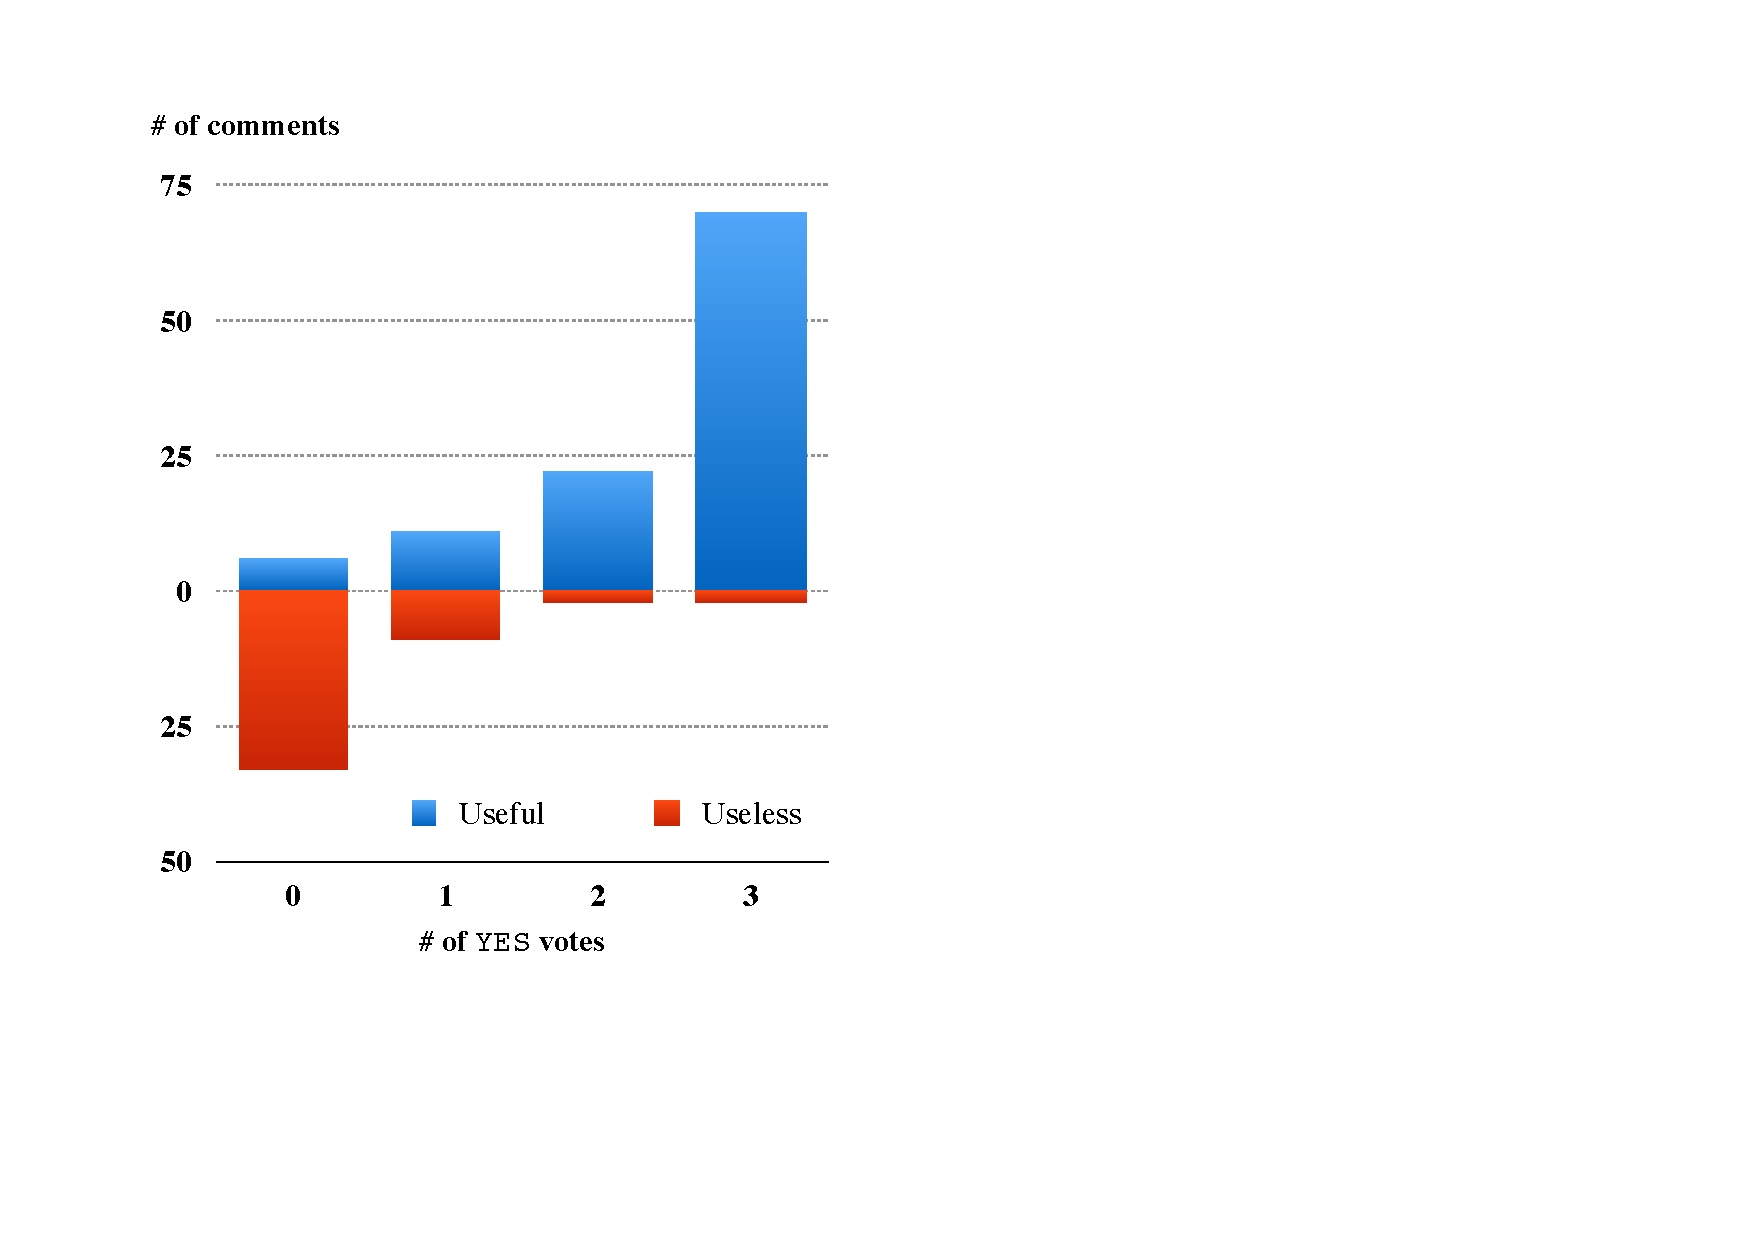
\includegraphics[width=2.5in]{posneg}
%\caption{The amount of comments by score classified by the binary classifier.}
%\label{fig:binary}
%\end{figure}

\subsection{Can other text mining techniques be used to classify discussions?}
To find relevance between comments and the corresponding commit message,
topic modeling technique can be used, as the study of \cite{Barua2012a}.
This technique discovers topics for a given collection of documents.
However, in MCR context, the documents generally are very short statements and discussions, which makes it unsuitable for LDA. 
Nevertheless, we have tried applying Latent Dirichlet Allocation (LDA, a well-known topic modeling technique) model on our data set.
As expected, LDA generated ambiguous topics with many unrelated keywords. Again, as discussed above, there is simply not enough information since the content of the documents are too short, and thus is insufficient for LDA to correctly determine the topic. Others techniques could be investigated in the future to improve results.

%\subsection{Reasons of Classification}
% reasons for classification as useful or not useful

%\subsection{What decisions are made during the manual classification?}
%During manual comment usefulness assessment, we recorded the participants' rationale to verify that the comments are actually technically or little direct contribute to the proposed changes. We can summarize that most of reason for \texttt{YES} voting are: the comments 1) contain new information 2) contain constructive suggestions, 3) discuss directly to the proposed changes, and 4) discuss the technical matters. For \texttt{NO} voting, we can summarize that the comments 1) are chatting (just communication), 2) talking about matters unrelated to the proposed changes, 3) discuss about process workflow and supporting system (e.g. Git and Gerrit).

%During the training process, reasons for the judgment are recorded. Examples of reasons for positive comments include:
%
%\begin{itemize}
%	\item they contain new information;
%	\item they contain constructive suggestions;
%	\item they discuss directly about the change; and
%	\item they discuss technical matters.
%\end{itemize}
%
%Examples of reasons for negative comments include:
%
%\begin{itemize}
%	\item chatting (i.e. no new information, just communication);
%	\item not discussing directly about the change;
%	\item discussing about the process workflow; and
%	\item discussing about Git or Gerrit itself.
%\end{itemize}

\subsection{Can the determined thresholds in this study be used to other projects?}

In this study, we determined the similarity conditions using a training set from the Qt project and the results show that the conditions can indeed classify usefulness of comments.
However, we have no basis for believing that the threshold values obtained for one project would apply equally well for another project. To apply our approach on other projects, a new training set is still required which implies additional manual assessment.
This limits the practicality of application our our method to projects with a large enough number of comments, where the classification effort saved overcomes the training costs.
To fully automate this approach, we have to investigate the use of similarity conditions for many other different projects. Thus, additional studies are needed to improve our approach and potentially identify invariant conditions for similarly and usefulness. 

%
%Secondly, owing to the subjective assessment of usefulness, this representation fundamentally implies supervised classification requiring nontrivial training data to define representative classification sets. This decreases the cost-effectiveness and limits the practicality of application to projects with a large enough number of comments, where the classification effort saved overcomes the training costs.


